% ---------------------------------------------------------------------------
% Revised draft: A Representation-Centred Evaluation of Latent Diffusion for
% Afrikaans Text Generation (BSc Honours, Wits CSAM).
%
% Build in the TACL template folder (needs tacl2021v1.sty and acl_natbib.bst):
%   xelatex main && bibtex main && xelatex main && xelatex main
% pdfLaTeX also works.
%
% Conventions used in this file
%   \textbf{[XX: ...]}    result or fact still to be supplied; never estimate it
%   \textbf{[CITE: ...]}  suggested citation not yet verified; never cite as is
%   \textbf{[tool, version]} etc.  blanks for the author to fill in
%   E1--E12               experiments listed in the change log / placeholder list
% Search for "[XX:" and "[CITE:" before submission: neither may remain.
% ---------------------------------------------------------------------------
\documentclass[11pt,a4paper]{article}
\usepackage[acceptedWithA]{tacl2021v1}
\usepackage{iftex}
\ifPDFTeX
  \usepackage[utf8]{inputenc}
  \usepackage[T1]{fontenc}
\fi
\usepackage{times}
\usepackage{latexsym}
\usepackage{amsmath}
\usepackage{amssymb}
\usepackage{booktabs}
\usepackage{tabularx}
\usepackage{graphicx}
\usepackage{adjustbox}
\usepackage{url}
\usepackage{microtype}

\title{A Representation-Centred Evaluation of Latent Diffusion\\for Afrikaans Text Generation}

\author{Hadi Butt\\
School of Computer Science and Applied Mathematics\\
University of the Witwatersrand, Johannesburg}

\date{}

\begin{document}
\maketitle

% Abstract.
\begin{abstract}
Latent diffusion generates text by denoising in a continuous space and decoding the result, so every sample passes through the autoencoder that defines that space. We test what this means for unconditional Afrikaans generation on the NCHLT corpus, using an mT5-base encoder--decoder adapted with a Perceiver bottleneck and two diffusion denoisers trained with five seeds each. The autoencoder reproduces only 11 of 81 held-out passages exactly and keeps 21 of 33 numerals; shuffling latents across documents shows that the decoder uses the latent, not that the latent preserves the passage. Generation scores do not reveal this. The larger denoiser lowers external mGPT perplexity from 51.31 to 48.61, and both sizes score better than a small autoregressive model trained from scratch, although after length standardisation the smaller one's advantage is not clear under either mGPT or a second Afrikaans scorer. Random latents decoded by the same decoder reach similar raw perplexity, yet only 5.5\% of their outputs are identified as Afrikaans. Retraining the full decoder raises reconstruction chrF only from 67.70 to 70.05, but a follow-up autoencoder with all parameters trained reconstructs 73 of 103 reserve passages exactly, against 19 for the original. Generation scores alone therefore cannot certify latent text generation: reconstruction fidelity has to be measured with them.
\end{abstract}

% ===========================================================================
\section{Introduction}
% ===========================================================================

A government notice states that the Departement van Maatskaplike Dienste en Armoedeverligting (Social Services and Poverty Alleviation) offers 44 bursaries a year, 20 of them for social development. Encoded into a latent and decoded again by an Afrikaans text autoencoder, the passage keeps 44, loses 20, and the department becomes ``Maatskaplike Ontwikkeling'' (Social Development; Appendix~\ref{app:examples}). Latent text diffusion generates text through such an autoencoder: a denoiser produces a latent, and a decoder turns it into words \citep{lovelace2023latent}. A sample can contain only what the decoder can express from a latent. In unconditional generation there is no source passage to compare against, so scores on generated text cannot show whether the autoencoder preserves content.

Latent text diffusion has been evaluated mainly on English and other high-resource benchmarks, by scoring generated text \citep{li2022diffusionlm,gong2023diffuseq,lovelace2023latent}. We found no study that tests whether its autoencoder preserves passages when adapted with limited in-domain data; \citet{lovelace2023latent} report reconstruction for English only. Afrikaans is an informative case. The NCHLT Clean Afrikaans Text Corpus provides documented, licensed government-domain text \citep{eiselen2014developing}, but only about 1.2 million training words, while Afrikaans is covered by a pretrained multilingual encoder--decoder, mT5 \citep{xue2021mt5}, and an external scorer, mGPT \citep{shliazhko2024mgpt}. The setting is therefore limited in-domain adaptation on top of large multilingual pretraining, not a model learning Afrikaans from the corpus alone.

We adapt mT5-base with a Perceiver bottleneck, following \citet{lovelace2023latent}, train two denoiser sizes with five seeds each, and evaluate the autoencoder before the generator. We ask three questions:
\begin{enumerate}
\item \textbf{RQ1:} What implementation and scaling constraints does a reduced English reproduction of the pipeline identify before the Afrikaans results are interpreted?
\item \textbf{RQ2:} Do autoencoders adapted to NCHLT Afrikaans preserve enough of a passage for faithful reconstruction?
\item \textbf{RQ3:} Does Afrikaans latent diffusion compare credibly with an autoregressive (AR) baseline under mGPT perplexity, diversity and repetition diagnostics, and tokenisation fertility?
\end{enumerate}

We call the system credible if its reconstructions preserve content, its mGPT perplexity is at most 1.20 times that of the AR baseline, and its outputs show no severe repetition or loss of diversity. These criteria were fixed before the experiments; the 1.20 ratio is a decision rule, not a validated measure of quality. The AR baseline shares the corpus and tokeniser but is a small model trained from scratch and sampled with nucleus sampling, whereas the diffusion system decodes with a pretrained decoder and beam search (Table~\ref{tab:conditions}). The comparison therefore sets two systems against each other, not two generation mechanisms. Appendix~\ref{app:deviations} lists every departure from the original design.

Our central finding is that favourable generation scores and unfaithful reconstruction coexist in the same system, and that the generation scores alone could not have revealed it. The contributions are:
\begin{enumerate}
\item A reconstruction analysis that separates use of the latent from preservation of the passage. Shuffling latents across documents raises teacher-forced cross-entropy from 1.079 to 8.319, so the decoder uses the latent; yet only 11 of 81 held-out passages are reconstructed exactly and 21 of 33 numerals survive (\S\ref{sec:res-recon}). Retraining the decoder alone raises chrF from 67.70 to 70.05, below a threshold fixed in advance (\S\ref{sec:res-interventions}).
\item Evidence that generation scores could not have shown this. Random latents decoded by the same decoder score 50.36 on validation, close to the diffusion samples (53.07 and 50.02), although only 5.5\% of their outputs are identified as Afrikaans. Across five seeds per size, the larger denoiser lowers test mGPT perplexity from 51.31 to 48.61, and both sizes score below a small AR baseline (validation ratios 0.6458 and 0.6087); after length standardisation, the smaller one's advantage is not clear under either mGPT or a second Afrikaans scorer (\S\ref{sec:res-gen}, \S\ref{sec:res-language}).
\item A follow-up autoencoder screen, with selection rules fixed in advance, showing that the reconstruction failure is not inherent to the setting. An autoencoder with all parameters trained, more Afrikaans data and longer latents reconstructs 73 of 103 unseen reserve passages exactly, against 19 for the original, with chrF 98.70 against 68.32; most of the gain is associated with training all parameters (\S\ref{sec:res-aescreen}). Its effect on generation has not yet been measured.
\end{enumerate}

The study covers one corpus, one domain and one language, and uses automatic measures only; no human evaluation was conducted.

% ===========================================================================
\section{Related work}
% ===========================================================================

\paragraph{Diffusion for text.}
Diffusion models generate by reversing a gradual noising process \citep{ho2020denoising,nichol2021improved}. For text, the discreteness of tokens has been handled by diffusing over discrete states \citep{austin2021structured}, over continuous word embeddings \citep{li2022diffusionlm,gong2023diffuseq} \citep{strudel2022self} \citep{dieleman2022continuous}, or with continuous models trained for likelihood \citep{gulrajani2023likelihood}. Latent diffusion instead denoises in the latent space of an autoencoder \citep{rombach2022high}. \citet{lovelace2023latent} apply this to language by compressing the states of a pretrained encoder--decoder, and \citet{zhang2023planner} extend it to paragraphs. Our architecture follows \citet{lovelace2023latent}, and their separation of autoencoding from generation sets the order of our evaluation.

\paragraph{Latent text autoencoders.}
A latent diffusion model can generate only what its decoder can express from a latent. Sentence variational autoencoders showed that a strong decoder may ignore its latent altogether \citep{bowman2016generating}; pretraining both sides of the autoencoder reduces this \citep{li2020optimus}, and bottleneck autoencoders built on pretrained transformers trade compression against reconstruction \citep{montero2021sentence}. Our autoencoder is not variational, so posterior collapse is not the mechanism at issue. The shared question is whether the latent carries the passage. We test it directly, with a shuffled-latent control, passage-level checks, and a comparison of autoencoders that train different parts of the model.

\paragraph{Evaluating open-ended generation.}
Open-ended generation has no reference output, so it is usually scored with an external language model and with diversity and repetition statistics. Probability and quality can disagree: beam search produces text that language models rate as highly probable but that differs from human text \citep{holtzman2020curious} \citep{meister2020beam}, and distribution-level measures were proposed partly for this reason \citep{pillutla2021mauve}. Any automatic metric needs validating for the use it is put to \citep{reiter2018structured}. We therefore pair mGPT perplexity \citep{shliazhko2024mgpt} with reconstruction measures and latent controls, and use chrF \citep{popovic2015chrf} only for paired reconstruction, where a reference exists.

\paragraph{Afrikaans and African-language NLP.}
Resources and evaluation tools for African languages are unevenly distributed \citep{joshi2020state,nekoto2020participatory}. Models pretrained on modest African-language data can be competitive \citep{ogueji2021small}, dedicated multilingual models widen coverage \citep{adebara2023serengeti}, and tokenisers that fragment words raise cost and lower accuracy \citep{lundin2025token}. Afrikaans-specific pretrained encoders exist \citep{ralethe2020adaptation}. We found no evaluation of diffusion-based generation for Afrikaans; this paper evaluates one, with the autoencoder examined separately from the generator.

% ===========================================================================
\section{Data and method}
\label{sec:method}
% ===========================================================================

\subsection{Corpus}
NCHLT Afrikaans contains government-domain text distributed by CTexT, North-West University, under CC BY 2.5 South Africa \citep{eiselen2014developing}; we use the clean 2.0 distribution (Appendix~\ref{app:data}). Preprocessing applies NFC and whitespace normalisation, conservative boilerplate removal and contact masking, then splits text into passages of at most 50 whitespace words, at punctuation where possible. Passages shorter than three words and exact duplicates after normalisation are removed; no language-identification filter is applied. Source documents are assigned with seed 42 to approximately 80/10/10 partitions, giving 47,767 training, 5,905 validation and 5,692 test passages from 2,005, 251 and 251 documents. No document or passage is shared across splits, although some 12-word sequences are (Appendix~\ref{app:data}).

We keep the mT5 tokeniser (250,100 entries, 128-token input cap) instead of training a SentencePiece vocabulary \citep{kudo2018sentencepiece} on NCHLT as proposed, because the pretrained embeddings depend on it. Validation fertility is 1.933 tokens per whitespace word, including special tokens.

\subsection{Autoencoder and diffusion}
Following \citet{lovelace2023latent}, the mT5-base encoder \citep{xue2021mt5} feeds a three-layer Perceiver \citep{jaegle2021perceiver} that compresses its states to $z_0 \in \mathbb{R}^{32\times 64}$, and a reconstruction map passes the latent to the mT5 decoder. Each non-zero latent vector is rescaled to norm eight. Adaptation trains the Perceiver components, the final decoder block and the final layer norm with teacher-forced cross-entropy (CE); all other weights stay frozen. We use the checkpoint at update 30,500 (AdamW, learning rate $10^{-4}$, effective batch eight, BF16), which continued an earlier pilot run (Appendix~\ref{app:training}). The code is a fork of the official implementation of \citet{lovelace2023latent}, extended for the NCHLT data, the mT5 tokeniser, and the training and evaluation described here.

For $t \sim \mathcal{U}(0,1)$ and Gaussian noise $\epsilon$, the signal variance is $a(t) = \max\{\cos^2(\pi t/2), 10^{-9}\}$ \citep{nichol2021improved}, and the denoiser is trained on
\begin{equation}
z_t = \sqrt{a(t)}\,z_0 + \sqrt{1-a(t)}\,\epsilon
\end{equation}
to predict the velocity $v_t = \sqrt{a(t)}\,\epsilon - \sqrt{1-a(t)}\,z_0$ \citep{salimans2022progressive} under mean squared error. This objective is not a likelihood over text. Self-conditioning \citep{chen2023analog} is applied with probability 0.5; training rescales the self-conditioning estimate to norm eight, but sampling does not (\S\ref{sec:limitations}).

\subsection{Systems compared}
Table~\ref{tab:conditions} summarises the systems. The small and large denoisers have width, depth and heads of 256/4/4 and 768/12/12, with one and three dense connections, dropout 0.1 and scale--shift conditioning, so several architectural settings change together. Both train with AdamW at $2\times10^{-4}$, 1,000 warm-up updates, cosine decay, gradient clipping at one and an exponential moving average (EMA) of weights with decay 0.9999, for at most 381 epochs. Every two epochs, EMA velocity MSE is measured on a fixed 2,048-passage validation probe, and the checkpoint with the lowest value is kept; stopping uses a separate patience rule (Appendix~\ref{app:training}). Each run samples latents with 250 DDPM steps \citep{ho2020denoising} and decodes them with beam search (four beams, length 5--128 tokens, repetition penalty 1.2, no repeated token trigrams). Each run produces 1,000 unconditional samples for validation and 1,000 for testing; the label names the role of the sample set, not any conditioning.

The AR baseline is a GPT-style model with four layers, width 256, four heads and tied embeddings, trained from random initialisation on the same splits with the same tokeniser. We use its checkpoint at update 60,000 of 157,529, selected on validation CE. It produces 256 samples from the start token with nucleus sampling ($p = 0.95$, temperature one, up to 127 new tokens), compared with the first 256 validation samples of each diffusion run. We do not decode the AR model with beam search: from a fixed start token, deterministic beam search returns the same output for every sample.

As a decoder-only control, we decode 1,000 Gaussian latents, each of the 32 slot vectors rescaled to norm eight, with the same decoder and beam settings, on the validation side only. This shows what the decoder produces from latents that carry no learned distribution.

\begin{table*}[t]
\centering
\small
\begin{adjustbox}{max width=\textwidth}
\begin{tabular}{llll}
\toprule
Condition & Small diffusion & Large diffusion & AR baseline \\
\midrule
Pretrained weights & Adapted mT5 & Same adapted mT5 & None (random initialisation) \\
Generator parameters & 8.10M & 187.98M & 67.22M \\
Training seeds & 42--46 & 42--46 & 42 \\
Precision / effective batch & FP32 / up to 64 & FP32 / up to 64 & BF16 / 8 \\
Exposure at selection & 288--306 epochs & 172--180 epochs & 480,000 sampled passages \\
Recorded training time & 2.93--3.13 h & 7.19--7.85 h & 4.52 h \\
Text decoding & Beam 4, constrained & Beam 4, constrained & Nucleus, $p=0.95$, temperature 1 \\
\bottomrule
\end{tabular}
\end{adjustbox}
\caption{Comparison conditions (RQ3). All systems use the same splits and tokeniser. Diffusion parameter counts exclude the shared autoencoder; the AR count includes its tied 250,100-entry embedding, so counts are not whole-system equivalents. Training times cover training and checkpoint selection on an RTX PRO 6000 Blackwell and exclude pretraining and autoencoder training. AR passages are sampled with replacement, so they are not complete epochs.}
\label{tab:conditions}
\end{table*}

% ===========================================================================
\section{Evaluation}
\label{sec:evaluation}
% ===========================================================================

\subsection{Reconstruction}
Teacher-forced CE measures prediction given the reference prefix; free-running reconstruction measures the full encode--decode path without it. For free-running output we report exact matches, mean sentence chrF \citep{popovic2015chrf}, and recall and precision of numerals against the tokenised input. Numeral matching is a string comparison and does not test numerical meaning. The main diagnostic uses 81 validation passages from 64 documents, at most two per document, all within the input cap. As a control, each passage's latent is replaced by that of a passage from another document in the same length bin, which breaks the link to the source while keeping realistic latent values. Earlier evaluations on 1,024 passages per split supply teacher-forced accuracy and exact-match rates. All 81 reconstructions were also labelled against the three content checks set in the proposal: named entities and content words preserved, main clause structure recognisable, and no unsupported lexical material. The labels were produced by an AI assistant that saw each source beside its reconstruction; they are an AI-assisted reading, not verified by the author or an Afrikaans reader.

\subsection{Generation}
All generated and human text is scored with mGPT in FP32, with a 512-token window and stride 256; each output is scored separately, prefixed with the scorer's beginning-of-sequence token, and every token is scored once. Perplexity for a sample set is
\begin{equation}
\mathrm{PPL} = \exp\Bigl(\textstyle\sum_i \mathrm{NLL}_i \big/ \sum_i n_i\Bigr),
\end{equation}
where $n_i$ counts scored tokens in sample $i$. It is token-weighted, not a mean of per-sample perplexities, and is not the generator's own likelihood. We also report mean length in whitespace words, distinct-$n$ (unique over total word $n$-grams within a sample set), the mean per-output fraction of repeated word trigrams, outputs that exactly match a training passage after NFC normalisation, case folding and whitespace collapsing, and the share of outputs identified as Afrikaans by GlotLID v3 \citep{kargaran2023glotlid}, taking the top label; outputs are also checked against the LibreOffice \texttt{af\_ZA} Hunspell dictionary (Appendix~\ref{app:language}). Human test passages are scored in the same way. Scorer and metric settings are in Appendix~\ref{app:scoring}. As a second scorer we use Goldfish, a monolingual Afrikaans model trained on 1\,GB of text \citep{chang2024goldfish}. Its tokeniser differs from mGPT's, so absolute values are never compared across scorers. Its model card does not list NCHLT among its Afrikaans sources. One of those sources, the Glot500 collection, includes NCHLT corpora at collection level; whether any NCHLT Afrikaans text reached the Afrikaans model is not documented, so overlap with our data cannot be ruled out. For comparisons between systems, perplexity is also length-standardised: per-band mean log-loss over four word-length bands (1--10, 11--20, 21--35 and 36 or more words) is reweighted to the human length distribution (weights 0.140, 0.223, 0.349 and 0.288) and exponentiated. A bank needs at least 20 outputs in every band.

\subsection{Uncertainty and data use}
Means and sample standard deviations are over five training runs. The large-minus-small perplexity difference is bootstrapped over runs without pairing, since equal seed numbers do not make outputs comparable; because five runs per arm is few for a bootstrap, we also report a Welch interval and an exact permutation test over all 252 divisions of the ten run means into two groups of five. Intervals for the AR ratio resample diffusion runs and their outputs and the outputs of the single AR checkpoint, so they omit AR and autoencoder training variation. Reconstruction intervals resample documents, keeping each source paired with its output. All bootstraps use 10,000 replicates, and all intervals are exploratory.

Benchmark checkpoints were selected on validation data only, but the test set was exposed during the wider project. The original autoencoder's reconstruction metrics on the first 1,024 test passages were reported to the author on 19 September and discussed in later diagnostic planning. On 9 October the five-seed diffusion test perplexities were reported and, at the author's request, an AI assistant rated 20 test-generation outputs from each configuration against 20 earlier samples; these ratings were unblinded and are not reported as results. From 23 October, reanalysis of the existing test banks was treated as secondary analysis of an exposed benchmark, with models and decoder frozen. Later diagnostic and reporting choices followed this exposure, so the test results are not a fresh confirmatory test. The decoder interventions below use only the 81 development passages; a 103-passage reserve from 64 other validation documents was not used.

\subsection{Decoder interventions}
After the benchmark was frozen, we tried three changes on the 81 development passages, each with a threshold fixed before it ran: decoding without the trigram ban (+2 chrF with a positive lower confidence bound, losing at most two percentage points of numeral recall); retraining the last two or all twelve decoder blocks; and retraining the full decoder with or without dropout (+3 chrF and at least 14 of 81 exact matches for both retraining experiments). Retraining used one seed and kept the encoder, Perceiver, embeddings, output projection and diffusion model frozen. Generation was to be re-evaluated only for a change that passed (Appendix~\ref{app:interventions}).

% ===========================================================================
\section{Results}
\label{sec:results}
% ===========================================================================

\subsection{Reconstruction: the decoder uses the latent but does not preserve the passage}
\label{sec:res-recon}

\begin{table}[t]
\centering
\small
\setlength{\tabcolsep}{4pt}
\begin{adjustbox}{max width=\columnwidth}
\begin{tabular}{lcc}
\toprule
Measure & Correct & Shuffled \\
\midrule
Teacher-forced CE & 1.079 & 8.319 \\
Mean sentence chrF & 67.70 & 12.84 \\
Exact reconstructions & 11/81 & 0/81 \\
Numerals recovered & 21/33 & 0/33 \\
Numeral precision & 0.840 & 0.000 \\
Outputs at length cap & 0/81 & 0/81 \\
All three content checks (AI-assisted) & 26/81 & -- \\
\bottomrule
\end{tabular}
\end{adjustbox}
\caption{Reconstruction of the same 81 validation passages (64 documents) from correct or shuffled latents (RQ2). Numeral counts are out of 33 numerals in the sources, not passages. All inputs are within the input cap.}
\label{tab:recon}
\end{table}

With correct latents, teacher-forced CE is 1.079; with shuffled latents it is 8.319, a difference of 7.240 (document-bootstrap 95\% CI [6.605, 7.933]), and chrF falls from 67.70 to 12.84 (Table~\ref{tab:recon}). The decoder therefore relies on source-specific information in the latent. The encode--decode path still loses content: only 11 of 81 passages are reconstructed exactly, and 21 of 33 source numerals survive. All inputs are within the cap and no output reaches the length limit, so neither truncation nor non-termination explains the errors. The earlier 1,024-passage evaluations agree: teacher-forced token accuracy is 82.75\% on validation and 80.59\% on test, but exact reconstruction is 12.21\% and 7.23\%.

The errors change content (Appendix~\ref{app:examples}). In one passage, 44 survives but 20 is lost, and the department name ``Maatskaplike Dienste en Armoedeverligting'' becomes ``Maatskaplike Ontwikkeling''. In another, ``regulering'' (regulation) becomes ``betaling'' (payment) and ``Regeringsdepartement'' (government department) becomes ``Regeringskommissie'' (government commission). In the AI-assisted reading, 55 of the 81 passages (68\%) fail at least one check: 52 lose a named entity or content word, 19 lose the main clause structure, and 55 contain unsupported material. The labeller treated some changes leniently, for example passing \emph{Ministerie} (ministry) rendered as \emph{Minister} and a question that lost \emph{MIV} (HIV); counting any change to a named entity, number or key noun as a failure raises the count to 62 (77\%). The first and third checks largely overlap, because a substituted word is usually counted both as lost and as unsupported.

\subsection{Generation: better scores that cannot certify the system}
\label{sec:res-gen}

\begin{table*}[t]
\centering
\small
\setlength{\tabcolsep}{4pt}
\begin{adjustbox}{max width=\textwidth}
\begin{tabular}{lccccccc}
\toprule
& \multicolumn{2}{c}{Validation, 256 samples} & \multicolumn{5}{c}{Test, 1,000 samples per run} \\
\cmidrule(lr){2-3}\cmidrule(lr){4-8}
System & PPL & Ratio to AR & PPL & Mean words & Distinct-2 & Train copies & Afrikaans \\
\midrule
Human text & 32.82\textsuperscript{a} & -- & 33.62 & 27.66 & 0.6796 & 0/1,000 & 98.2\%\textsuperscript{c} \\
Random latents, same decoder & 57.60\textsuperscript{b} & 0.7009 & -- & -- & -- & -- & -- \\
AR, nucleus sampling & 82.18 & -- & -- & -- & -- & -- & 95.3\%\textsuperscript{c} \\
Small diffusion (5 runs) & 53.07 & 0.6458 & 51.31 $\pm$ 1.49 & 29.30 & 0.6606 & 5/5,000 & 96.3 $\pm$ 0.9\%\textsuperscript{c} \\
Large diffusion (5 runs) & 50.02 & 0.6087 & 48.61 $\pm$ 0.91 & 26.34 & 0.6903 & 79/5,000 & 97.2 $\pm$ 0.2\%\textsuperscript{c} \\
\bottomrule
\end{tabular}
\end{adjustbox}
\caption{Generation results (RQ3). Diffusion values are means over five runs, with sample standard deviation where shown; copy counts aggregate the five runs. Ratio 95\% intervals: small [0.5813, 0.7148], large [0.5477, 0.6736]; they omit AR and autoencoder training variation, as there is one AR run. Distinct-2 standard deviations are 0.00513 (small) and 0.00283 (large). Human text values are for 1,000 sampled passages per split, not the full splits; \textsuperscript{a}all 1,000 validation passages. \textsuperscript{b}First 256 of 1,000 Gaussian latents decoded on 30 October; this control was not run on the test side (all 1,000: 50.36, mean 37.34 words, distinct-2 0.8674, no training copies). \textsuperscript{c}Share of outputs whose top GlotLID label is \texttt{afr\_Latn}, measured on validation outputs (human: 4,825 passages of at most 128 tokens, 95\% document-bootstrap interval 96.5--98.7\%; diffusion: 1,000 outputs per run; AR: the 256 validation samples); test outputs were not classified. The AR baseline was evaluated on validation only, so its test cells are empty. ``Afrikaans'' is the share of outputs identified as Afrikaans.}
\label{tab:generation}
\end{table*}

\paragraph{Denoiser size.}
Across five runs each, the larger denoiser lowers test perplexity from 51.31 to 48.61 (difference $-$2.704, a 5.27\% reduction; run-bootstrap 95\% CI [$-$4.076, $-$1.334]; Welch 95\% CI [$-$4.567, $-$0.841]; exact permutation $p = 6/252 = 0.024$) and test velocity MSE from 0.5011 to 0.4512 (Table~\ref{tab:generation}). Because width, depth, heads, dense connections and training exposure change together, this is the effect of the larger configuration as a whole, not of capacity alone. Its outputs are shorter (26.34 against 29.30 words) and copy a training passage exactly more often (79 against 5 of 5,000). Shorter human passages score higher perplexity (Figure~\ref{fig:length}), so shorter outputs would, if anything, raise the larger model's score; on validation outputs, removing exact training copies (5 of 5,000 small and 52 of 5,000 large outputs) leaves mean mGPT perplexity almost unchanged (51.94 to 51.93 and 49.60 to 49.56), so copies do not explain the gap. Test outputs were not rescored. Repeated-trigram fractions are low for both, $1.30\times10^{-5}$ and $2.91\times10^{-5}$, partly because decoding bans repeated token trigrams. Both configurations produce 6 of 5,000 outputs at the length cap and none empty.

\paragraph{AR comparison.}
On 256 validation samples, mGPT perplexity is 82.18 for the AR baseline and 53.07 and 50.02 for small and large diffusion, giving ratios of 0.6458 and 0.6087, well within the 1.20 threshold. The AR model's own validation perplexity, 36.41, is a different quantity and is not comparable. The comparison sets a pretrained decoder with beam search against a small model trained from scratch with nucleus sampling (Table~\ref{tab:conditions}), so it compares two systems rather than two generation mechanisms. Random latents decoded by the same decoder score 57.60 on the first 256 (ratio 0.7009) and 50.36 on all 1,000. Random latents therefore score about as well as small diffusion, although their outputs are longer (37.34 words on average) and longer outputs score lower on this scorer; mGPT perplexity alone does not show that the denoiser adds to the decoder.

\paragraph{Human reference and length.}
Human test passages score 33.62, so diffusion samples lie between human text and the AR baseline. The scorer is strongly length-dependent: human passages of 1--10 words score 240.83, and those of 36 words or more score 25.93 (Figure~\ref{fig:length}). Both diffusion sizes score above human text in every band longer than ten words, so the length mix does not explain the gap to human text. In the two shortest length bands, the AR baseline scores better than small diffusion on validation (1--10 words: 281.32 against a five-run mean of 346.00; 11--20 words: 78.99 against 86.49), while large diffusion scores 205.52 and 68.00. Aggregate perplexity therefore depends on the length mix of each sample set.

\begin{figure}[t]
\centering
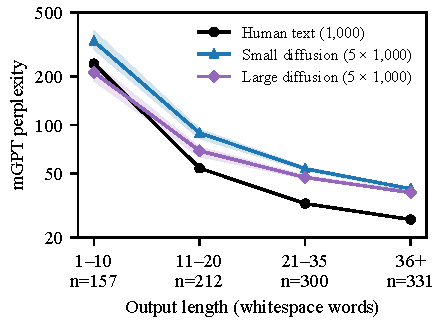
\includegraphics[width=\columnwidth]{figures/length_bands.pdf}
\caption{mGPT perplexity by output length on the test split, log scale: 1,000 human passages (counts per band under each label) and five runs of 1,000 outputs for each diffusion size (line: mean of the run values; shading: range). The AR baseline is omitted because it was evaluated on validation only.}
\label{fig:length}
\end{figure}

\subsection{Generation: language, shared phrasing and a second scorer}
\label{sec:res-language}

Table~\ref{tab:language} adds checks made after the main results, under a protocol fixed before they were run. Most diffusion outputs are identified as Afrikaans: 96.3\% for the small configuration and 97.2\% for the large, against 98.2\% for human validation text (95\% interval 96.5--98.7\%). The small configuration falls just below that interval, and the shortfall is concentrated in outputs of ten words or fewer, where identification is least reliable (Appendix~\ref{app:language}). Words not recognised by the Afrikaans dictionary make up 5.8\% and 5.9\% of diffusion tokens, slightly above the human interval (3.2--5.7\%). The historical AR sample has 95.3\% identified as Afrikaans and 5.3\% unrecognised tokens.

The random-latent control shows why these checks matter. Its mGPT perplexity is close to the diffusion values (Table~\ref{tab:generation}), yet only 5.5\% of its outputs are identified as Afrikaans (26.4\% as Dutch) and 70\% of its tokens are not in the dictionary. Under Goldfish its raw perplexity (56.1) is lower than that of either diffusion configuration. Length-standardised mGPT perplexity ranks it last, but neither scorer's raw perplexity on its own detects that the output is not Afrikaans.

Diffusion outputs share fewer word 4-grams with the training split than held-out human text does: 8.7\% (small) and 11.8\% (large), against 14.4\% for human text (95\% interval 10.2--19.4\%). The large configuration has more outputs in which at least 90\% of 4-grams occur in training (4.3\% against 1.1\% for the small configuration and 1.5\% for human text), in line with its higher copy count. The historical AR sample has 5.5\%.

Under Goldfish, every comparison points in the same direction as under mGPT (Table~\ref{tab:language}). The large-minus-small difference and the large configuration's advantage over the historical AR sample are confirmed under both scorers. After length standardisation, the small configuration's advantage over that sample is not clear under either scorer: both intervals contain no difference. The comparison against recombined training slots (C3) cannot be made, because C3 has only two outputs of ten words or fewer. Across 33 banks the two scorers' standardised perplexities have Spearman $\rho = 0.83$.

\begin{table*}[t]
\centering
\small
\begin{adjustbox}{max width=\textwidth}
\begin{tabular}{lcccccc}
\toprule
& \multicolumn{2}{c}{Language (Part A)} & \multicolumn{2}{c}{Training overlap (Part B)} & \multicolumn{2}{c}{Standardised perplexity} \\
\cmidrule(lr){2-3}\cmidrule(lr){4-5}\cmidrule(lr){6-7}
Bank & Afrikaans & Unrecognised tokens & 4-gram overlap & High-overlap rows & mGPT & Goldfish \\
\midrule
Human validation (4,825) & 98.2 [96.5, 98.7] & 4.3 [3.2, 5.7] & 14.4 [10.2, 19.4] & 1.5 & -- & -- \\
Human, scored subset (811) & 97.9 & 4.2 & 15.7 & 1.5 & 41.55 & 64.60 \\
Reconstructions of that subset & 98.5 & 4.8 & 11.3 & 0.6 & 52.00 & 103.5 \\
Small diffusion (5 $\times$ 1,000) & 96.3 $\pm$ 0.9 & 5.8 $\pm$ 0.3 & 8.7 $\pm$ 0.4 & 1.1 $\pm$ 0.4 & 71.29 $\pm$ 1.73 & 194.3 $\pm$ 4.2 \\
Large diffusion (5 $\times$ 1,000) & 97.2 $\pm$ 0.2 & 5.9 $\pm$ 0.2 & 11.8 $\pm$ 0.7 & 4.3 $\pm$ 0.4 & 59.58 $\pm$ 0.78 & 148.1 $\pm$ 4.4 \\
AR, nucleus sampling (256) & 95.3 & 5.3 & 15.8 & 5.5 & 80.52 & 203.7 \\
C1 random latents (1,000) & 5.5 & 70.5 & 0.0 & 0.0 & 107.6 & 98.4 \\
C2 projected Gaussian (1,000) & 99.7 & 4.6 & 8.3 & 0.0 & 63.57 & 172.5 \\
C3 recombined slots (1,000) & 98.9 & 5.0 & 7.2 & 0.0 & n/s & n/s \\
\midrule
\multicolumn{7}{l}{Comparisons: log ratio of standardised perplexity [95\% interval] (ratio)} \\
\midrule
& \multicolumn{3}{c}{mGPT} & \multicolumn{3}{c}{Goldfish} \\
Large vs small & \multicolumn{3}{c}{$-$0.179 [$-$0.209, $-$0.150] (0.84)} & \multicolumn{3}{c}{$-$0.272 [$-$0.310, $-$0.234] (0.76)} \\
Small vs AR & \multicolumn{3}{c}{$-$0.122 [$-$0.270, 0.026] (0.89)} & \multicolumn{3}{c}{$-$0.047 [$-$0.246, 0.151] (0.95)} \\
Large vs AR & \multicolumn{3}{c}{$-$0.301 [$-$0.446, $-$0.156] (0.74)} & \multicolumn{3}{c}{$-$0.319 [$-$0.520, $-$0.118] (0.73)} \\
Each size vs C3 & \multicolumn{3}{c}{insufficient band support} & \multicolumn{3}{c}{insufficient band support} \\
\bottomrule
\end{tabular}
\end{adjustbox}
\caption{Language identification, dictionary recognition, training overlap and standardised perplexity on validation outputs. Values are percentages except perplexities; diffusion values are means $\pm$ sample SD over five runs. Afrikaans: share with GlotLID top label \texttt{afr\_Latn}. Unrecognised tokens: share of word tokens, excluding all-capital acronyms, not accepted by the \texttt{af\_ZA} dictionary. 4-gram overlap: share of word 4-grams that occur in the training split. High-overlap rows: outputs with at least four 4-grams, of which at least 90\% occur in training. Bracketed human intervals come from 2,000 document-bootstrap replicates. n/s: fails band support (two outputs of ten words or fewer). Large vs small uses a Welch interval; comparisons with AR use $t_4(0.9875)$ with the AR sample's bootstrap variance. Overlap is described relative to human text and is not evidence of memorisation.}
\label{tab:language}
\end{table*}

To test whether the AR baseline was disadvantaged by its sampling settings, it was resampled under 18 settings: temperature 0.8, 0.9 or 1.0, top-$p$ 0.90, 0.95 or 1.00, with and without the diffusion decoder's repetition constraints (1,000 outputs each; Appendix~\ref{app:argrid}). A setting qualified for a tuned comparison only if it was at least as diverse as the least diverse diffusion run (distinct-2 at least 0.664 and unigram entropy at least 9.227 bits) and produced no more exact training copies than the diffusion run with the most (13). Six settings met both diversity conditions, but every setting produced between 36 and 112 exact training copies per 1,000 outputs, so none qualified and no tuned-AR comparison is made. Lower temperature and top-$p$ lower AR perplexity (from 125.0 to 43.4) at the cost of diversity and more copies (Figure~\ref{fig:frontier}).

\begin{figure*}[t]
\centering
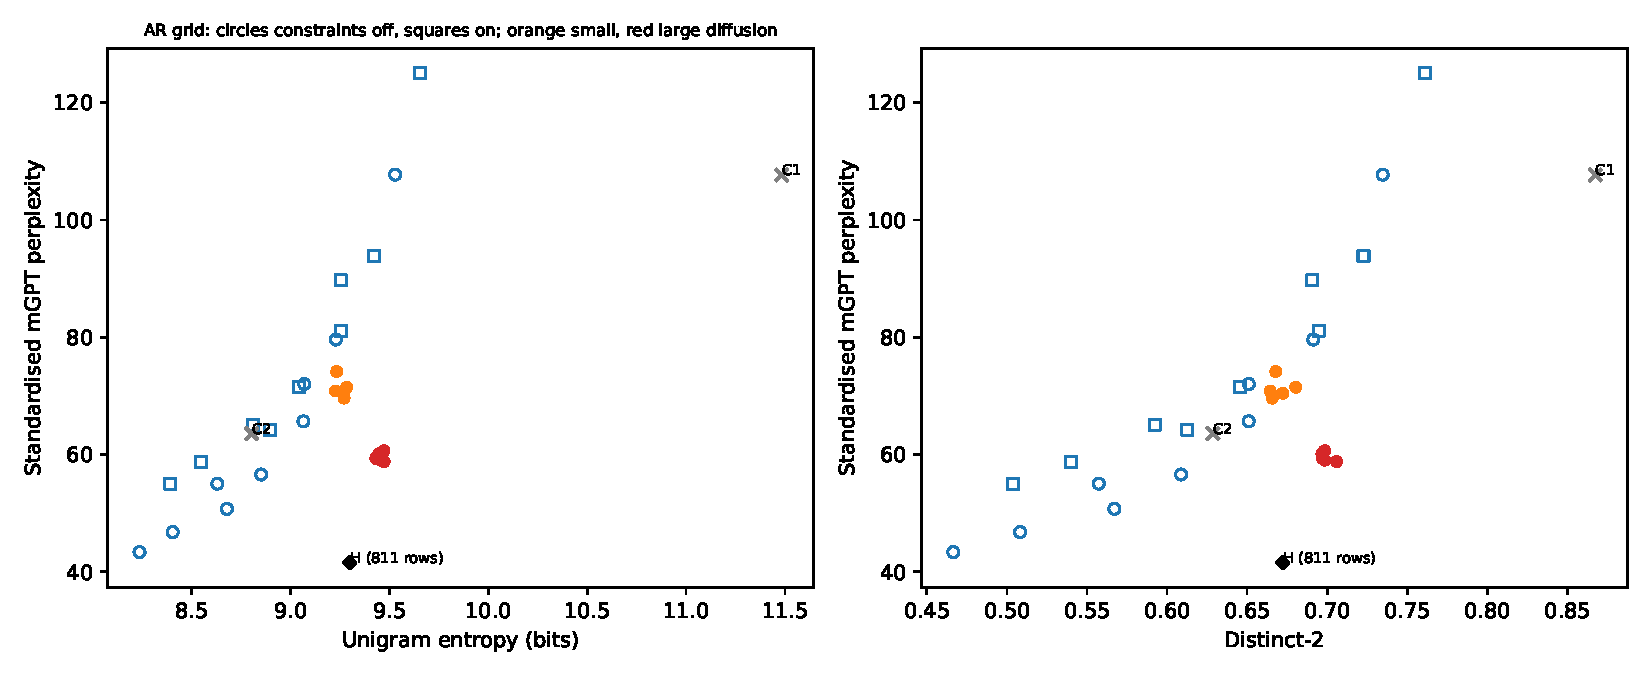
\includegraphics[width=\textwidth]{figures/frontier.pdf}
\caption{Standardised mGPT perplexity against unigram entropy (left) and distinct-2 (right) on validation outputs. Open circles: AR settings without repetition constraints; open squares: with them. Orange: small diffusion runs; red: large diffusion runs; crosses: latent controls C1--C3; diamond: human reference (811 outputs, so its entropy is not comparable). No AR setting qualified for a tuned comparison.}
\label{fig:frontier}
\end{figure*}

\subsection{Decoder interventions: gains below threshold}
\label{sec:res-interventions}

\begin{table*}[t]
\centering
\small
\setlength{\tabcolsep}{4pt}
\begin{adjustbox}{max width=\textwidth}
\begin{tabular}{lcccccl}
\toprule
Change & Update & chrF & Exact & Numerals & Generation PPL & Outcome \\
\midrule
None (original decoder) & 0 & 67.70 & 11 & 21 & 51.31 / 48.61 & Reference \\
Decoding: no trigram ban & -- & 68.62 & 14 & 19 & -- & Below threshold \\
Retrain last two blocks & 0 & 67.70 & 11 & 21 & -- & No eligible gain \\
Retrain all twelve blocks & 26,520 & 70.05 & 13 & 25 & -- & Below threshold \\
All twelve, dropout off & 9,720 & 69.86 & 13 & 24 & -- & Control arm \\
All twelve, dropout 0.1 & 3,720 & 68.44 & 9 & 21 & -- & Below threshold \\
\bottomrule
\end{tabular}
\end{adjustbox}
\caption{Decoder interventions on the 81 development passages (RQ2), run after the benchmark was frozen. Exact matches are out of 81 passages and numerals out of 33. Rows show the checkpoint chosen by the pre-set rule, not necessarily the highest chrF. Retraining thresholds were 70.7005 chrF and 14 exact matches. The two retraining experiments ran 26,620 and 16,920 updates per arm. Generation PPL is test perplexity (small / large); generation was not re-evaluated with the retrained decoders.}
\label{tab:interventions}
\end{table*}

No change met its threshold (Table~\ref{tab:interventions}). Removing the trigram ban raised chrF by 0.918 (paired document-bootstrap 95\% CI [$-$0.110, 2.016]) and exact matches to 14, but numerals fell from 21 to 19 of 33 and repeated word trigrams rose from none to 80. Retraining the full decoder gave the largest gain: chrF rose from 67.70 to 70.05 and numerals from 21 to 25 of 33 (chrF change 2.35, paired document-bootstrap 95\% CI [0.78, 3.96], conditional on the selected checkpoint), but chrF stayed below 70.7005 and exact matches reached 13 against the required 14. Its selected checkpoint (update 26,520) lies near the end of its 26,620-update budget, so the run was limited by budget rather than shown to have converged. Its teacher-forced CE, 1.337, is higher than the original 1.079, so the two selection criteria disagree. Retraining only the last two blocks found no eligible checkpoint better than the original, and dropout 0.1 did worse than dropout off (68.44 against 69.86 chrF). As no change passed, generation was not re-evaluated in the original protocol, and no generation scores are reported for the retrained decoders.

\subsection{Follow-up: training the whole autoencoder}
\label{sec:res-aescreen}

To test whether the reconstruction failure is inherent to the setting, we trained four new autoencoders under a protocol fixed before training (Table~\ref{tab:aescreen}). All four follow the full mT5-base recipe of \citet{lovelace2023latent}: every parameter is trained, at effective batch 128 and learning rate $10^{-4}$, whereas the original trained only the Perceiver, the final decoder block and the final layer norm. The arms cross two factors: NCHLT alone or NCHLT with 511,155 further words of government-domain Afrikaans (Gov-ZA cabinet statements and Vuk'uzenzele), and 32 or 64 latent slots. The extra text was deduplicated against all NCHLT splits, and any document sharing a 12-word sequence with NCHLT validation or test was removed; diffusion still trains on NCHLT only. Arms were ranked by cross-entropy on a 663-passage selection panel, and the winner was evaluated once, with the original, on 103 reserve passages held back since 22 October. The reserve is disjoint from every panel used for selection but comes from the validation split, which was used earlier in the project.

\begin{table}[t]
\centering
\small
\begin{adjustbox}{max width=\columnwidth}
\begin{tabular}{llccccc}
\toprule
Arm & Data & Slots & Sel.\ CE & Exact & chrF & Numerals \\
\midrule
Original & NCHLT & 32 & 0.802 & 26 & 69.24 & 0.62 \\
A & NCHLT & 32 & 0.066 & 118 & 96.35 & 0.94 \\
B & NCHLT & 64 & 0.018 & 126 & 97.89 & 1.00 \\
C & + extra & 32 & 0.066 & 121 & 96.51 & 0.99 \\
D & + extra & 64 & 0.015 & 134 & 98.20 & 1.00 \\
\midrule
\multicolumn{7}{l}{Reserve, 103 passages} \\
Original & NCHLT & 32 & -- & 19 & 68.32 & 0.77 \\
D (winner) & + extra & 64 & -- & 73 & 98.70 & 1.00 \\
\bottomrule
\end{tabular}
\end{adjustbox}
\caption{Autoencoder screen. Upper rows: 194-passage comparison panel (exact matches out of 194). Sel.\ CE: teacher-forced cross-entropy on the 663-passage selection panel. Numerals: recall of source numerals. All arms train every parameter; the original trains only part of the model. Every arm stopped at its six-hour cap after about 3,500 of a planned 10,000 updates.}
\label{tab:aescreen}
\end{table}

Every arm reached its six-hour cap after about 3,500 of the planned 10,000 updates, so none was trained to completion, yet all four improve sharply on the original. On the comparison panel, training all parameters at the original latent size raises exact matches from 26 to 118 of 194 (difference 47.4 points, 95\% CI [40.4, 54.7]) and chrF from 69.24 to 96.35. Doubling the latent length adds 4.1 points [0.0, 8.3] without the extra data and 6.7 [3.3, 10.5] with it; the extra data add 1.5 [$-$1.4, 4.6] and 4.1 [1.1, 7.4] points. Arm D won and met all three reserve thresholds fixed in advance: 73 of 103 exact against 19 (difference 52.4 points, CI [42.5, 63.3]; at least 10 required), chrF 98.70 against 68.32 (difference 30.4, CI [24.7, 36.6]; at least 3 required), and numeral recall 1.00 against 0.77. Long passages remain the hardest: the winner reconstructs 1 of 15 long reserve passages exactly, against 45 of 47 short ones. Intervals are paired document bootstraps with 10,000 replicates.

Diffusion trained on the winning autoencoder, with the same denoisers, seeds and scoring as the main benchmark, was not complete for this version, so no generation results are reported for it. Its protocol fixes in advance what would count as improved generation, including a random-latent control for the new decoder. The screen shows that the original autoencoder was under-trained, not that the setting rules out faithful reconstruction; it does not show that better reconstruction yields better generation.

% ===========================================================================
\section{Discussion}
\label{sec:discussion}
% ===========================================================================

\paragraph{Verdict on the research questions.}
\emph{RQ1 is partly answered.} A reduced English control (ROCStories with BART, 5,000 updates at an effective batch of 32) reached validation token accuracy of 93.26\% and 11 of 128 exact reconstructions (8.59\%, 95\% interval 4.9--14.7\%); on test the figures were 93.11\% and 10 of 128. The autoencoder training code therefore learns to reconstruct English. The shorter runs identified two constraints: at a batch of two, 1,000 updates gave 11.29\% token accuracy and no exact reconstructions, and one BF16 run at an effective batch of 16 diverged to an undefined loss. The control used neither the proposed OpenWebText data nor the published 50,000-update, batch-256 schedule, and the Afrikaans autoencoder uses mT5 rather than BART, so it cannot rule out every implementation fault specific to the Afrikaans configuration. \emph{RQ2's criterion is not met.} The proposal treats the representation as insufficient if reconstructions are visibly unfaithful under its three checks, and the reconstructions in \S\ref{sec:res-recon} change names, numerals and content words. The follow-up screen shows that this failure belongs to the original autoencoder, not to the setting: an autoencoder trained in full meets every reconstruction threshold set for it (\S\ref{sec:res-aescreen}). The verdict below concerns the system as tested. \emph{RQ3 is met only on its numerical component.} The perplexity ratios are within 1.20, and repetition and diversity show no collapse. However, the comparison is not matched, and mGPT is unstable across length bands on human text (240.83 against 25.93), so under the proposal's own rule the perplexity comparison counts only as a weak diagnostic. Two further checks narrow what the numerical result means. After length standardisation, the small configuration's advantage over the AR sample is not clear under either mGPT or Goldfish (Table~\ref{tab:language}), and perplexity under neither scorer flags random-latent output that is mostly not Afrikaans. Most diffusion outputs are identified as Afrikaans, at rates close to human text. Fertility is reported descriptively (1.933 tokens per word), since an inherited tokeniser leaves nothing to compare it with. \emph{The hypothesis is not supported}, because credibility required adequate reconstruction.

\paragraph{Why scores and fidelity diverge.}
Every sample, from either denoiser, passes through the same pretrained mT5 decoder with beam search, a repetition penalty and a trigram ban. Beam search favours high-probability continuations \citep{holtzman2020curious}, and both the decoder and the scorer were pretrained on large multilingual corpora \citep{xue2021mt5,shliazhko2024mgpt}, and both cover Afrikaans: mT5 through mC4, mGPT through Wikipedia and C4. Such a decoder may produce text that the scorer rates highly from a latent that preserves little of any particular passage. Two measurements test this. Random latents decoded by the same decoder score 50.36 on validation, against 53.07 and 50.02 for the diffusion samples (Table~\ref{tab:generation}), so the decoder alone reaches diffusion-level raw perplexity. Reconstructions of the 81 development passages score 70.67 against 61.76 for their sources (log-perplexity difference 95\% CI [0.001, 0.258]), so the decoder does not simply pull text towards high-probability Afrikaans. The random-latent outputs also show that a good raw score does not imply Afrikaans text: only 5.5\% are identified as Afrikaans, and length-standardised perplexity ranks them last (\S\ref{sec:res-language}). Raw perplexity therefore cannot separate what the denoiser contributes from what the decoder contributes, and it does not detect output that is not Afrikaans.
The conclusion does not depend on this explanation: a better denoiser changes which latents reach the decoder but cannot restore what the autoencoder fails to preserve, so better generation scores cannot be read as better representation.

\paragraph{Under-adaptation or bottleneck?}
The reconstruction errors could come from a latent too small to hold a passage (a bottleneck) or from an autoencoder that has not been trained enough to use the latent it has (under-adaptation). The evidence favours under-adaptation. Only the Perceiver, the final decoder block and the final layer norm were trained, with the encoder frozen, and the selected checkpoint follows 30,500 updates at effective batch eight on 47,767 training passages, after an earlier pilot whose cumulative training is not recoverable. Unfreezing the full decoder raised chrF from 67.70 to 70.05 and numerals from 21 to 25 of 33, with the best checkpoint near the end of its budget. The gap between teacher-forced token accuracy (82.75\%) and exact reconstruction (12.21\%) shows how small per-token errors compound over a passage, but it does not show whether the missing information is absent from the latent. A bottleneck predicts that errors grow with passage length at fixed latent size and that a larger latent helps more than longer training. Exact matches do fall with length: on the 103 reserve passages the original autoencoder reconstructs 16 of 47 short, 3 of 41 medium and none of 15 long passages exactly (up to 32, 33--64 and 65--128 tokens). The follow-up screen (\S\ref{sec:res-aescreen}) tested both explanations directly. Training all parameters at the original latent size raised exact matches on a 194-passage comparison panel by 47 percentage points, while doubling the latent length added 4 to 7 points. Under-adaptation therefore accounts for most of the failure, with a smaller length-related bottleneck that a longer latent partly relieves.

\paragraph{Implication.}
For latent text diffusion in a new language, reconstruction fidelity should be measured at passage level and reported before generation scores are interpreted, and generation scores should be set against human text and a decoder-only control.

% ===========================================================================
\section{Limitations}
\label{sec:limitations}
% ===========================================================================

\paragraph{Scope.}
The study covers one administrative corpus, one language and one task. It says nothing about conversational or literary Afrikaans, or about other African languages, many of which differ in morphology and tokenisation \citep{lundin2025token}. Some 12-word sequences are shared across splits, and the training data were not filtered by language, and training text was not screened with language identification.

\paragraph{Comparisons.}
The diffusion system inherits mT5 pretraining; the AR baseline does not. They also differ in decoding, precision and compute (Table~\ref{tab:conditions}). The AR budget was set against an earlier diffusion run, not the final five-seed suite, and the small configuration was designated the primary comparator after budgets were reconciled. The comparison therefore cannot attribute differences to diffusion versus autoregression. An mT5 model fine-tuned as an unconditional generator, decoded identically, would remove the largest confound.

\paragraph{Measurement.}
mGPT perplexity depends strongly on length and is not the generator's likelihood. chrF and numeral matching are surface measures, and low repetition is partly enforced by decoding. As planned in the proposal, there was no human evaluation with participants; the examples in \S\ref{sec:res-recon} and the samples inspected during the project were read with AI assistance, and no Afrikaans reader verified those readings.

\paragraph{Uncertainty and data use.}
The five seeds per configuration are conditional on one autoencoder, one data split and one AR run, and each decoder intervention used one seed. Reusing the 81 development passages makes intervention gains exploratory, and earlier inspection of test outputs means the test set is not untouched (\S\ref{sec:evaluation}).

\paragraph{Implementation.}
The autoencoder continued a pilot whose optimiser history is not recoverable, so whole-system training cost is not reported. The English control was a reduced ROCStories run, not the proposed OpenWebText reproduction. Training rescales the self-conditioning estimate but sampling does not; the effect of this mismatch on generation was not tested.

% ===========================================================================
\section{Conclusion}
% ===========================================================================

Adapting latent diffusion to Afrikaans produced samples that an external language model scores well, better than a small autoregressive baseline and better again with a larger denoiser, from an autoencoder that does not reproduce its inputs faithfully. Random latents passed through the same decoder scored almost as well, and the scores could not have revealed the reconstruction failure. Retraining the decoder alone did not close the gap; training the whole autoencoder did, on passages held back for that test. Whether better reconstruction also yields better generation remains to be measured. For latent text diffusion in a new language, reconstruction fidelity should be measured and reported before generation scores are interpreted.

\section*{AI use}
AI assistance supported artifact auditing, retrospective analysis, sample inspection, drafting and LaTeX preparation. AI-assisted inspection is not participant-based human evaluation; independent verification of the Afrikaans interpretations is not claimed. The author is responsible for the final claims and for completing the institution's required disclosure. Tool and model details should be recorded in that declaration; its submission is not established here.

\section*{Ethics}
The corpus is publicly licensed (CC BY 2.5 South Africa), and contact details were masked during preprocessing. No human participants were involved. Institutional ethics approval or exemption has not been verified and is not inferred from the absence of participants.

\section*{Data and code}
Code, configurations and research documentation are available at \url{https://github.com/hadibutt3560/afrikaans-latent-diffusion}, branch \texttt{main}. The claim-to-evidence register is in \path{docs/research/paper_revision_2026-10-26/EVIDENCE_REGISTER.md}. Model weights, raw corpora and complete generated sample banks are local artifacts excluded from Git; the repository alone does not contain all assets needed to reproduce the experiments.

\bibliographystyle{acl_natbib}
\bibliography{references}

% ===========================================================================
\appendix
% ===========================================================================

\section{Deviations from the proposal}
\label{app:deviations}

\begin{table*}[t]
\centering
\small
\begin{tabularx}{\textwidth}{@{}p{2.4cm}XXX@{}}
\toprule
Item & Proposal & This paper & Reason \\
\midrule
English control & OpenWebText, public Lovelace et al.\ code & ROCStories with BART, 5,000 updates at effective batch 32 & Supported upstream route; short sequences eased implementation checks; avoided OpenWebText preparation and compute. Reported as an implementation control, not a full reproduction \\
Tokeniser & SentencePiece BPE trained on NCHLT & mT5 tokeniser (250,100 entries) & Pretrained embeddings depend on it \\
AR baseline & Matched corpus, tokeniser, length and compute & Matched corpus and tokeniser & Training allowance set provisionally against the runtime of an earlier diffusion run, before the final five-seed benchmark; checkpoint kept after a later budget audit \\
Reconstruction inspection & Researcher checklist with three checks & Three examples (\S\ref{sec:res-recon}); all 81 labelled by an AI assistant, unverified & Planned assessment not completed during the main analysis; no reason is documented \\
mGPT on reconstructions & Planned & 81 diagnostic passages: sources 61.76, reconstructions 70.67 (log-perplexity difference 95\% CI [0.001, 0.258]) & -- \\
Distinct-1 & Planned & Test: 0.2229 $\pm$ 0.0039 (small), 0.2343 $\pm$ 0.0022 (large) & -- \\
Fertility analysis & English vs Afrikaans, linked to results & One Afrikaans value & Inherited tokeniser; no comparison possible \\
Generated-sample checklist & Researcher-side inspection & A local model judge, validated on a corruption test before use; both candidates failed, so no judge results are reported (Appendix~\ref{app:failedgates}). Unrecognised words read by an AI assistant (Appendix~\ref{app:language}) & Planned researcher assessment not completed; no reason is documented. Participant-based evaluation was outside the proposal, which does not remove this check \\
Additions & -- & Five seeds per configuration; shuffled-latent control; decoder interventions; reserve set & Stronger evidence than planned \\
AI use & ChatGPT for editing and LaTeX structure & Artifact auditing, analysis, inspection, drafting and LaTeX preparation; AI-assisted reading of 150 unrecognised words & Disclosed separately from human evaluation \\
\bottomrule
\end{tabularx}
\caption{Deviations from the research proposal.}
\label{tab:deviations}
\end{table*}

Table~\ref{tab:deviations} summarises the documented changes to the proposal's design.

\section{Data}
\label{app:data}

The catalogue resource is \url{https://hdl.handle.net/20.500.12185/293}. Its metadata lists version 1, while the local file names and preprocessing manifest identify clean 2.0; we treat these as possibly different releases. The acquisition date and release mapping are not documented, so local source hashes identify the material used. The documentation requires attribution to the Department of Arts and Culture and CTexT.

Split statistics are: training, 2,005 documents, 47,767 passages and 1,228,292 words; validation, 251, 5,905 and 158,331; test, 251, 5,692 and 158,332. These counts agree with the saved preprocessing statistics; the validation and test word totals do differ by one. Exact document and text overlap checks pass. Sampled 12-word sequences shared across splits number 418 (training/validation), 899 (training/test) and 184 (validation/test); these are shared sequences, not duplicate documents. The tokeniser audit finds no unknown tokens; 95 training, two validation and six test passages exceed the 128-token cap. Units are passages, not necessarily sentences.

\section{Training and selection}
\label{app:training}

\paragraph{Autoencoder.} The selected checkpoint is job 56531, update 30,500. Its continuation uses micro-batch one with accumulation eight, AdamW with betas (0.9, 0.999), weight decay 0.01, clipping at one, and a constant learning rate of $10^{-4}$ after 25 warm-up steps. Backbone dropout is disabled while gradients flow to the trained parameters. Selection evaluates a shuffled 128-example validation subset every 250 updates. The run resumes an earlier pilot whose optimiser history and cumulative compute are not recoverable.

\paragraph{Diffusion.} Micro-batch 16 with accumulation four (smaller final batches retained), AdamW with betas (0.9, 0.999), weight decay $10^{-6}$ and a 5\% learning-rate floor. The checkpoint with the strictly lowest probe MSE is kept. A relative improvement of 0.001 resets patience, and training stops after 12 checks without one, once at least 60 epochs have run. Validation noise seed is 18371; reported validation and test MSE use the full split with three noise repetitions. The ten runs are \texttt{small-seed42} to \texttt{small-seed46} and \texttt{published-seed42} to \texttt{published-seed46}, where ``published'' labels the large configuration. All ten are reported.

\paragraph{AR baseline.} Job 57759 selects update 60,000 of a 157,529-update run on a 128-example validation probe; the reported time covers the whole run. A checkpoint audit confirms strict loading and tokeniser equivalence. Samples use seeds 30,000--30,255.

\paragraph{English control.} The control used ROCStories with a frozen BART-base, a 64-token input, a batch of 8 with 4 accumulation steps (effective 32), BF16 and 5,000 updates, evaluated on 128 validation and 128 test examples at the final step. Validation CE was 0.239, token accuracy 93.26\% and exact reconstruction 11 of 128; test CE was 0.265, token accuracy 93.11\% and exact reconstruction 10 of 128. Validation exact reconstruction was 13 of 128 at step 4,500; the final step is reported rather than this peak. An earlier pilot at a batch of 2 reached validation CE 5.976, token accuracy 11.29\% and no exact reconstructions after 1,000 updates on 64 examples.

\section{Decoder interventions}
\label{app:interventions}

Both retraining experiments start from the original autoencoder, use AdamW at $2\times10^{-5}$, effective batch eight, FP32, seed 20261024, 100 warm-up updates and a constant learning rate, with matched data order within each experiment and dropout always off at evaluation. Job 74177 (RTX 8000) compares the last two decoder blocks with all twelve, dropout off, and stops at its budget. Job 75003 (RTX PRO 6000 Blackwell) compares full-decoder retraining with dropout off or 0.1 during training, and stops when neither arm gains 0.5 chrF over six paired checks after at least 12,000 updates. A checkpoint is eligible if it has no empty or capped reconstructions, numeral recall and precision within 0.02 of the original, and a repeated-trigram fraction within 0.005. Eligible checkpoints are ranked by chrF, then exact matches, then earlier update. To advance, a checkpoint needed +3 chrF over the original and at least 14 of 81 exact; all twelve blocks additionally needed +1 chrF over the best eligible two-block checkpoint, and dropout 0.1 needed to beat dropout off. Only the dropout 0.1 arm could advance in job 75003. Reserve confirmation and generation re-evaluation depended on advancing. Full trajectories are kept with the artefacts; neither experiment estimates seed variation.

\section{Scoring and environments}
\label{app:scoring}

The mGPT revision is \texttt{40897bd7c8b4\allowbreak 7a76802c4111\allowbreak 08ca6220438b\allowbreak 8b40}. Reconstruction chrF uses SacreBLEU 2.6.0 with character orders 1--6, no word $n$-grams, mixed case, no whitespace and effective order; the aggregate is mean sentence chrF, not corpus chrF. The reconstruction diagnostic sample uses seed 91427. The generation bootstrap seed is 20261023 and the decoding-intervention paired bootstrap seed is 91428. Shuffled-latent intervals are conditional on a fixed donor assignment. Training used PyTorch 2.7.1, CUDA 12.8 and Transformers 4.38.2; final scoring used PyTorch 2.11.0, CUDA 12.8 and Transformers 5.5.0 on an RTX 3060. Bitwise reproducibility across these environments was not tested. An evidence register maps each claim to files and SHA-256 hashes.

\section{Language and dictionary checks}
\label{app:language}

GlotLID v3 (\texttt{cis-lmu/glotlid}, revision \texttt{baa20d1}) classifies each output with line breaks replaced by spaces. Dictionary recognition uses the LibreOffice \texttt{af\_ZA} Hunspell files (commit \texttt{892f0f4}) through \texttt{spylls} 0.1.7, with Hunspell's own case rules. Tokens are NFC-normalised and matched by a pattern that keeps the article \emph{'n} whole; all-capital tokens of two or more letters are treated as acronyms and excluded. Including them raises the token rate to 4.6\% (human), 6.3\% (small), 6.5\% (large) and 5.5\% (AR). Type rates depend on bank size and are not compared across banks of different size.

\begin{table}[h]
\centering
\small
\begin{adjustbox}{max width=\columnwidth}
\begin{tabular}{lcccc}
\toprule
Words & 1--10 & 11--20 & 21--35 & 36+ \\
\midrule
Human validation & 88.7 & 98.9 & 99.6 & 100.0 \\
Small diffusion & 85.4 & 97.7 & 97.8 & 99.4 \\
Large diffusion & 89.0 & 97.8 & 99.0 & 99.4 \\
AR, nucleus & 88.9 & 98.8 & 98.1 & 100.0 \\
C1 random latents & 5.7 & 4.6 & 5.6 & 5.9 \\
\bottomrule
\end{tabular}
\end{adjustbox}
\caption{Share (\%) identified as Afrikaans by output length. Human band sizes: 620, 1,173, 1,677 and 1,355; AR: 90, 84, 54 and 28.}
\label{tab:lid-bands}
\end{table}

\paragraph{Manual check of unrecognised words.} 150 unrecognised token occurrences were drawn (seed 20261101): 50 from human text, 50 from the diffusion runs and 50 from the AR sample, with at most two occurrences of any word per group. They were shown in context, in random order and without their source. The labels were produced by an AI assistant (Claude), which knew the study's aims; this is an AI-assisted reading, not human evaluation, and the human manual check was not conducted. The labels file was hashed before the source key was joined. Of the 50 occurrences from each group, the reading labelled as valid Afrikaans (compounds, names and abbreviations the dictionary lacks) 39 from human text, 19 from diffusion and 29 from AR; as misspelt or malformed 8, 22 and 12; as not Afrikaans 2, 3 and 8; and 1, 6 and 1 as undecidable. Most unrecognised words in human text are therefore dictionary gaps, while nearly half of those in diffusion output are malformed words, which suggests the dictionary rate understates the difference in malformed words between diffusion and human text.

\paragraph{Second scorer and copies.} Goldfish (\texttt{goldfish-models/afr\_latn\_1000mb}, revision \texttt{27555fd}) scores every bank with the same code as mGPT. Removing exact training copies changes mean standardised perplexity by less than 0.5\% for either diffusion configuration under either scorer; for the AR sample (11 of 256 removed), mGPT standardised perplexity falls from 80.52 to 79.13 and Goldfish from 203.7 to 203.2. Word 8-gram overlap with training is 3.0\% for human text, 0.4\% (small), 2.4\% (large) and 3.4\% (AR). Overlap with the training split includes formulaic administrative phrasing that also recurs in held-out human text, so it is reported relative to human text and not as memorisation.

\section{AR sampling grid}
\label{app:argrid}

\begin{table}[h]
\centering
\small
\begin{adjustbox}{max width=\columnwidth}
\begin{tabular}{lcccc}
\toprule
Setting & mGPT (std.) & Distinct-2 & Entropy & Copies \\
\midrule
$T$0.8, $p$0.90 & 43.4 / 55.0 & 0.467 / 0.504 & 8.24 / 8.39 & 105 / 112 \\
$T$0.8, $p$0.95 & 46.8 / 58.7 & 0.508 / 0.540 & 8.40 / 8.55 & 87 / 89 \\
$T$0.8, $p$1.00 & 55.0 / 65.1 & 0.557 / 0.592 & 8.63 / 8.81 & 68 / 68 \\
$T$0.9, $p$0.90 & 50.7 / 64.2 & 0.567 / 0.613 & 8.68 / 8.90 & 84 / 76 \\
$T$0.9, $p$0.95 & 56.6 / 71.5 & 0.609 / 0.646 & 8.85 / 9.04 & 68 / 64 \\
$T$0.9, $p$1.00 & 72.0 / 89.7 & 0.651 / 0.691 & 9.07 / 9.25 & 49 / 46 \\
$T$1.0, $p$0.90 & 65.6 / 81.1 & 0.651 / 0.695 & 9.07 / 9.26 & 58 / 55 \\
$T$1.0, $p$0.95 & 79.6 / 93.8 & 0.691 / 0.723 & 9.23 / 9.42 & 46 / 46 \\
$T$1.0, $p$1.00 & 107.7 / 125.0 & 0.735 / 0.761 & 9.53 / 9.66 & 37 / 36 \\
\midrule
Qualifying floor & -- & $\geq$ 0.664 & $\geq$ 9.227 & $\leq$ 13 \\
\bottomrule
\end{tabular}
\end{adjustbox}
\caption{AR settings, 1,000 outputs each (seeds 30000--30999); each cell gives repetition constraints off / on. Entropy is unigram entropy in bits; copies are exact training copies. All settings meet band support; none meets the copy floor.}
\label{tab:argrid}
\end{table}

\section{Checks that did not pass validation}
\label{app:failedgates}

\paragraph{MAUVE: not reported, calibration gate failed.} MAUVE \citep{pillutla2021mauve} with LaBSE embeddings \citep{feng2022labse} was to be reported only if two disjoint halves of human validation text scored as near-identical. Over ten such splits of 1,000 passages each, the median was 0.140 (range 0.094--0.229) against a required 0.90, and changing the human reference draw moved the score by 0.211. The random-latent control scored 0.004, below every human split, and clustering variation was small (SD 0.017), but the measure does not recognise human text as matching human text on this corpus, so no system is compared with it.

\paragraph{Checklist judge: not reported, the judge failed validation.} A local model was to apply the proposal's generated-sample checklist (seven yes/no items; prompt in the protocol) after passing a corruption test: 900 items built from human passages, 150 left clean and 150 for each of five corruptions (word shuffle, broken word forms, repetition, truncation, and a splice of Dutch or English text from Universal Dependencies r2.18). A judge had to flag at least 80\% of every corruption, at most 20\% of clean passages and at most 2\% unparsed answers.

\begin{table}[h]
\centering
\small
\begin{adjustbox}{max width=\columnwidth}
\begin{tabular}{lcc}
\toprule
& Gemma 4 12B (Q4\_0) & Qwen3.5 9B (Q4\_K\_M) \\
\midrule
Clean passages flagged & 15.3 & 21.3 \\
Shuffle detected & 99.3 & 98.7 \\
Broken word forms detected & 70.0 & 86.7 \\
Repetition detected & 100.0 & 95.3 \\
Truncation detected & 82.0 & 80.0 \\
Splice detected & 99.3 & 97.3 \\
Unparsed answers & 0.0 & 0.0 \\
Random-latent outputs flagged & 100.0 & 100.0 \\
\midrule
Result & fails (word forms) & fails (clean rate) \\
\bottomrule
\end{tabular}
\end{adjustbox}
\caption{Judge validation on the selection half (\%). Both models ran in llama.cpp \texttt{b11630} with reasoning disabled. Neither passed, so the confirmation half was not rated and the judge was not applied to any system's outputs.}
\label{tab:judge}
\end{table}

\section{Reconstruction examples}
\label{app:examples}

The wording has been checked against the previously verified example source. In particular, ``Ontwikkeling-studiebeurse'' and ``derde-twintig'' occur in the saved text and are retained rather than corrected as typesetting artifacts.

The examples are the first stored rows in three disjoint categories, chosen to show one success and two kinds of failure; they do not estimate prevalence. Text is reproduced without correction. Each compares the model input with the original decoder's output.

\paragraph{Exact reconstruction (row 12).} Source: Wat Is Krediet Wat Is 'n Lening? Reconstruction: Wat Is Krediet Wat Is 'n Lening?

\paragraph{Numeral lost (row 4).} Source: Die Departement van Maatskaplike Dienste en Armoedeverligting bied elke jaar 44 beurse aan vir voltydse studie in Maatskaplike Werk. Vier-en-twintig van di\'e beurse word spesifiek aangebied vir manlike Maatskaplike Werkstudente, terwyl 20 van hulle vir Maatskaplike Ontwikkeling-studiebeurse is wat toegestaan word deur die Maatskaplike Ontwikkeling- en die Gesondheid- en Welsyns-SETA. Reconstruction: Die Departement van Maatskaplike Ontwikkeling bied elke jaar 44 beurse aan. Vier van die eerste - en derde-twintig beurs word spesifiek aangebied vir mans en vroue wat toegeken word aan die Maatskappy- en Welvaartstudies, terwyl die meeste van hierdie beursies word toegewys aan die Gesondheid en Lewensbeurse.

\paragraph{Content changed, no numerals (row 0).} Source: Die Provinsiale Regeringsdepartement van Vervoer en Openbare Werke is verantwoordelik vir regulering van die minibustaxibedryf in die provinsie. Die regulerende liggaam is die provinsiale taxikantoor wat by die volgende nommers geskakel kan word\ldots{} Reconstruction: Die Provinsiale Regeringskommissie van Vervoer en Openbare Werke is verantwoordelik vir die betaling van die minibushandel wat die provinsiale taxikantoor in die provinsie geskakel het. Die regulerende kantoor sal die nuwe taxikantoor aan die volgende taxikantoor geskakel word\ldots{}

\section{Generated samples}
\label{app:samples}

\textbf{Selection rule.} For each diffusion size we take the seed-42 run's test bank and rows 0, 500 and 999 in stored order; for the AR baseline, rows 0, 128 and 255 of its 256 validation samples; for random latents decoded by the same decoder, rows 0, 500 and 999 of the 1,000 validation decodes. The rule was fixed before the rows were read, and no row was replaced. Text is reproduced without correction, except that runs of characters from non-Latin scripts are shown as [\ldots]. The English glosses were written by an AI assistant and have not been verified by an Afrikaans reader; they are rough guides to content, not translations, and the samples illustrate outputs without estimating how common any feature is.

\paragraph{Small diffusion (test, seed-42 run; rows 0, 500, 999).}
\begin{itemize}\small
\item[0] \emph{Deur die Minister van Arbeid se KSG se Sekbondsertifikaatsaansgawes is die KOSTE 'n kombinasie van nuwe en amptelike fonds vir die Skool vir Baccalaurisieteikens verskaf. Dié projek is reeds op 60 dae gelede en is vanaf 1 Januarie 2006 vir gratis.}\\
Gloss (AI-assisted, unverified): Through the Minister of Labour's KSG's [garbled certificate term], the COST is a combination of new and official funds provided for the School for [garbled term]. This project is already 60 days ago and is free from 1 January 2006.
\item[500] \emph{wat word (in dié uitdrukking) ingestel word, wat grond gemaak word om graangebruik te voorsien, wat 'n aktuele uitslag is van die volgende twee hoofdoelwittes: Entrepreneurskap en die ontwikkeling van menslike werknemers.}\\
Gloss (AI-assisted, unverified): which is (in this expression) instituted, which land is made to provide grain use, which is a current result of the following two main objectives: entrepreneurship and the development of human employees.
\item[999] \emph{Sodra 'n gedeelte van ons Suid-Afrika van hierdie gebied voorsien word, moet die polisie nie langer as twee breide op hierdie plan het nie, want dit is nie die belangrikste om te onthou om dit te verstaan nie. Dit is ons oë vir ons wense om te antwoord nie.}\\
Gloss (AI-assisted, unverified): As soon as a part of our South Africa is supplied from this area, the police must not have more than two [unclear word] on this plan, because it is not the most important to remember to understand it. It is our eye for our wishes not to answer.
\end{itemize}

\paragraph{Large diffusion (test, seed-42 run; rows 0, 500, 999).}
\begin{itemize}\small
\item[0] \emph{Die Stadsraad het die volle R2,2 miljoen se wykstoekennings vir Sub-raad 14 goedgekeur. Die toekenning word gelykop tussen kapitaal- en beleggingsprojekte verdeel. Die volle wet word hoofsaaklik tussen kapitale- en klein-raads-projekte verhoog.}\\
Gloss (AI-assisted, unverified): The City Council approved the full R2.2 million of ward allocations for Sub-council 14. The allocation is divided equally between capital and investment projects. The full act is mainly increased between capital and small-council projects.
\item[500] \emph{sodat óf baie jongmense in Suid-Afrika verkoop word; en wat 'n bydrae word tot groter uitdagings in die landbousektor sal maak.}\\
Gloss (AI-assisted, unverified): so that either many young people in South Africa are sold; and which will make a contribution to greater challenges in the agricultural sector.
\item[999] \emph{Nie 'n provinsie waarin ons nie sy eerste dorpie op hierdie stadium sal staan nie, maar teken dat die polisie nie sy tweede strydrol op dieselfde stadium op die been sal gaan om te voort te gaan nie. Dit is die uitdaging om te volg op die belangstelling van ons boerdery op die grondwet op te volg.}\\
Gloss (AI-assisted, unverified): Not a province in which we will not stand its first village at this stage, but sign that the police will not get its second battle role on its feet at the same stage to continue. It is the challenge to follow up the interest of our farming on the constitution.
\end{itemize}

\paragraph{AR, nucleus sampling (validation, 256 samples; rows 0, 128, 255).}
\begin{itemize}\small
\item[0] \emph{Die nasionale handelsmerk was regtig besig om die Afrikaner te verbeter, met ander banke en ander rolspelers op plaaslike regering. Beskrywing van plaaslike regering en in die Wes-Kaap wil 'n plaaslike regering wees vir al die gemeenskapslede wat by die ander sektor besluit (wat uitgenooi is om volhoubare}\\
Gloss (AI-assisted, unverified): The national brand was really busy improving the Afrikaner, with other banks and other role-players in local government. Description of local government and in the Western Cape wants to be a local government for all the community members who decide in the other sector (who were invited to sustainable [cut off at the token cap]
\item[128] \emph{Verleenondersteuning aan almal: kerke en organisasies wat boere binnekort ons uitsette lewer.}\\
Gloss (AI-assisted, unverified): [Garbled compound meaning roughly "lend support"] to all: churches and organisations that soon deliver our outputs to farmers.
\item[255] \emph{Die datum waarop die huidige eienaar van die vuurwapen aanmeld, moet in paragraaf F 5 aangeteken word.}\\
Gloss (AI-assisted, unverified): The date on which the current owner of the firearm reports must be recorded in paragraph F 5.
\end{itemize}

\paragraph{Random latents, same decoder (validation, 1,000 samples; rows 0, 500, 999).}
\begin{itemize}\small
\item[0] \emph{\textless{}extra\_id\_0\textgreater{}ry d ry ry d na i ny d i n ry of ing,  i na tsident a n, ,  na , die , d  na si , na u i kwa i,, \textless{}extra\_id\_20\textgreater{} na ya d ,}\\
Gloss (AI-assisted, unverified): Not interpretable: letter fragments, punctuation and sentinel tokens.
\item[500] \emph{\textless{}extra\_id\_0\textgreater{}, a / de de de (.,9.,1 fees., enments., A}\\
Gloss (AI-assisted, unverified): Not interpretable: fragments, repeated function words and numerals.
\item[999] \emph{\textless{}extra\_id\_0\textgreater{} / a s n kodi o a rekord in[\ldots] ser orotique programme rekord. O[\ldots] POL za lisans online. [\ldots] word pro[\ldots]szelszel polli 18 lisans. 77 snomercial ne nada a \textless{}extra\_id\_20\textgreater{} ser or \textless{}extra\_id\_21\textgreater{}[\ldots] \textless{}extra\_id\_27\textgreater{} \textless{}extra\_id\_27\textgreater{} Standard. \textless{}extra\_id\_21\textgreater{} \textless{}extra\_id\_51\textgreater{} Standard. \textless{}extra\_id\_20\textgreater{} \textless{}extra\_id\_51\textgreater{} serandaane \textless{}extra\_id\_20\textgreater{} \textless{}extra\_id\_21\textgreater{} \textless{}extra\_id\_21\textgreater{} Standard \textless{}extra\_id\_27\textgreater{} serandaaner ser korone ko nada aan datum[\ldots]r [\ldots] naar \textless{}extra\_id\_21\textgreater{} deel \textless{}extra\_id\_21\textgreater{} international serotique seer ser or[\ldots] Europe ser anonymo in PRO 277 kroon konto ser on[\ldots] nomo CN rekord domain , ko \textless{}extra\_id\_39\textgreater{} Standard Standard O Junior profile [\ldots]}\\
Gloss (AI-assisted, unverified): Not interpretable: sentinel tokens and fragments of Afrikaans, English and other words, with characters from other scripts.
\end{itemize}


\end{document}
